\documentclass{beamer}

\usepackage{beamerthemesplit}
\usepackage{amsmath}
\usepackage{amsfonts}
\usepackage{amssymb}
\usepackage{qtree}
\usepackage{cancel}

\mode<presentation>
{
  \usetheme{Warsaw}
  % or ...

  %\setbeamercovered{transparent}
  % or whatever (possibly just delete it)
}


\usepackage[english]{babel}
% or whatever

\usepackage[latin1]{inputenc}
% or whatever

\usepackage{times}
\usepackage[T1]{fontenc}


%%%%%%%%% NEW COMMANDS %%%%%%%%%
\newcommand{\score}{{\it score}}
\newcommand{\fitness}{{\it fitness}}
\newcommand{\sizepenalty}{{\it sizePenalty}}
\newcommand{\pset}[1]{\Theta_i(#1)}
\newcommand{\argmax}[1]{\underset{#1}{\operatorname{argmax}}\ }
\newcommand{\argmin}[1]{\underset{#1}{\operatorname{argmin}}\ }
\newcommand{\stos}{f_i}
\newcommand{\stof}{g_i}


\title{Learning Server Overview}

\author{Nil Geisweiller}

\begin{document}

\frame
{
  \maketitle
}

\frame
{
  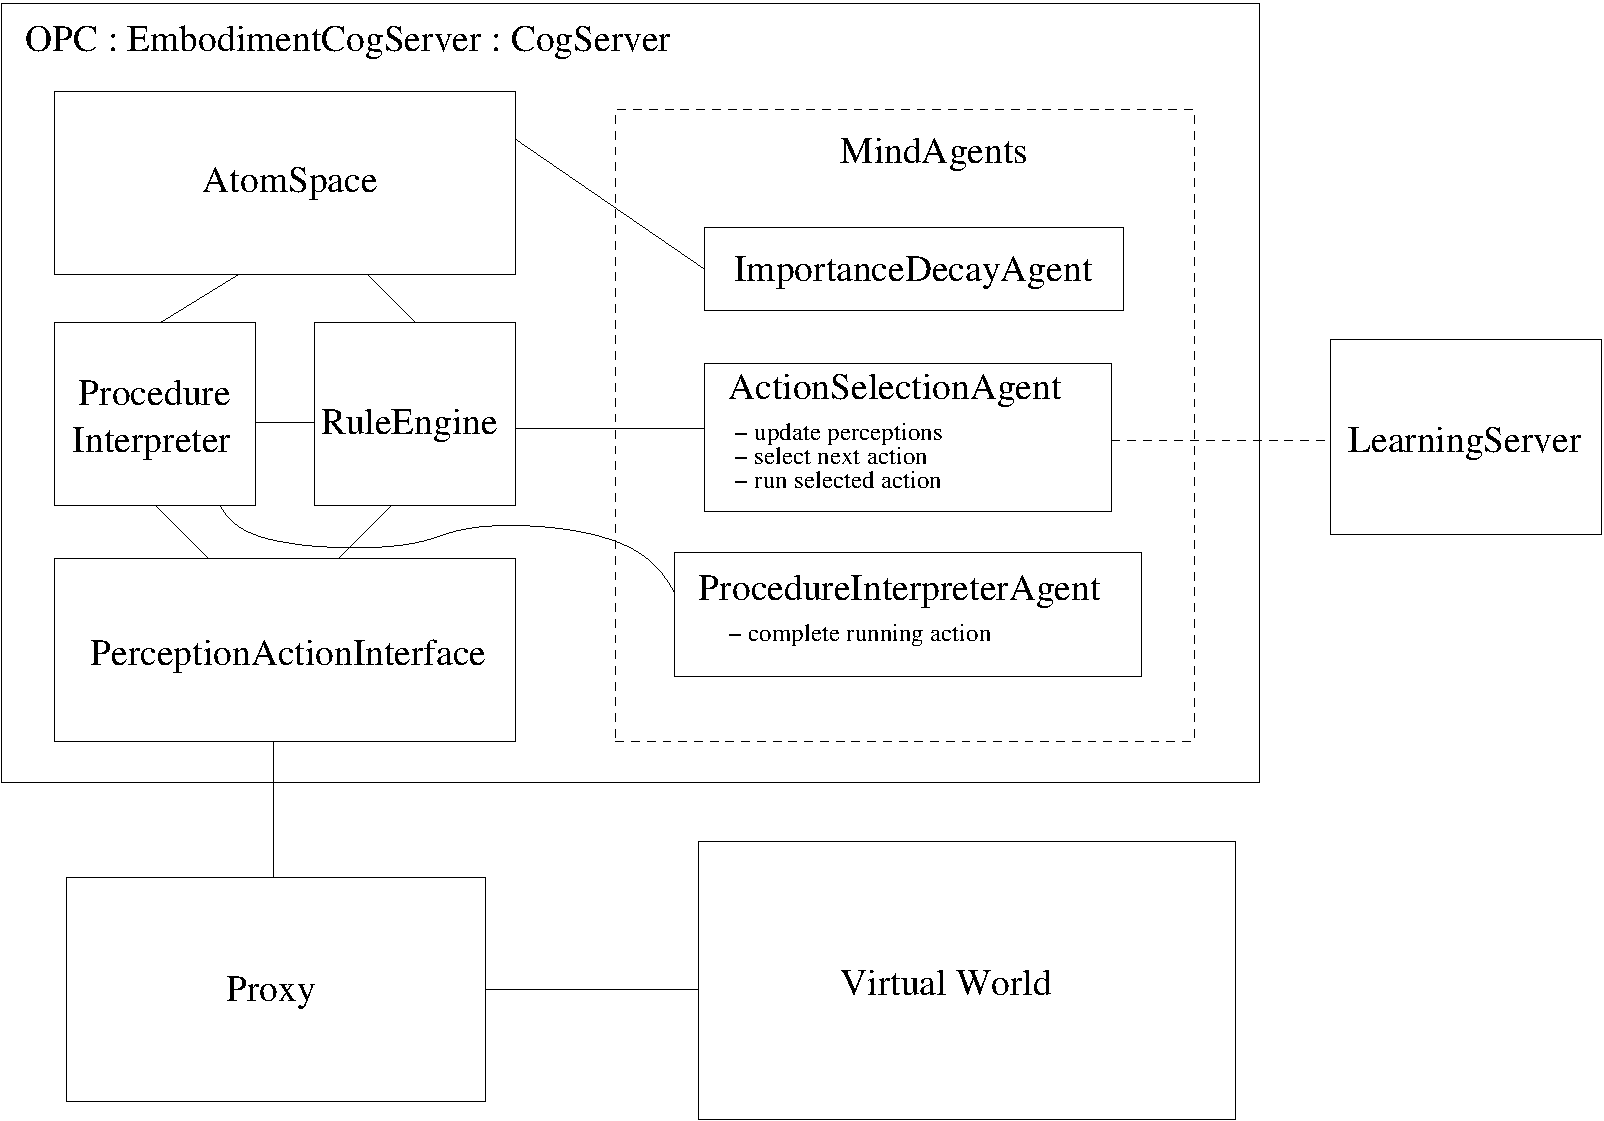
\includegraphics[scale=0.4]{OPC.pdf}
}

\frame
{
  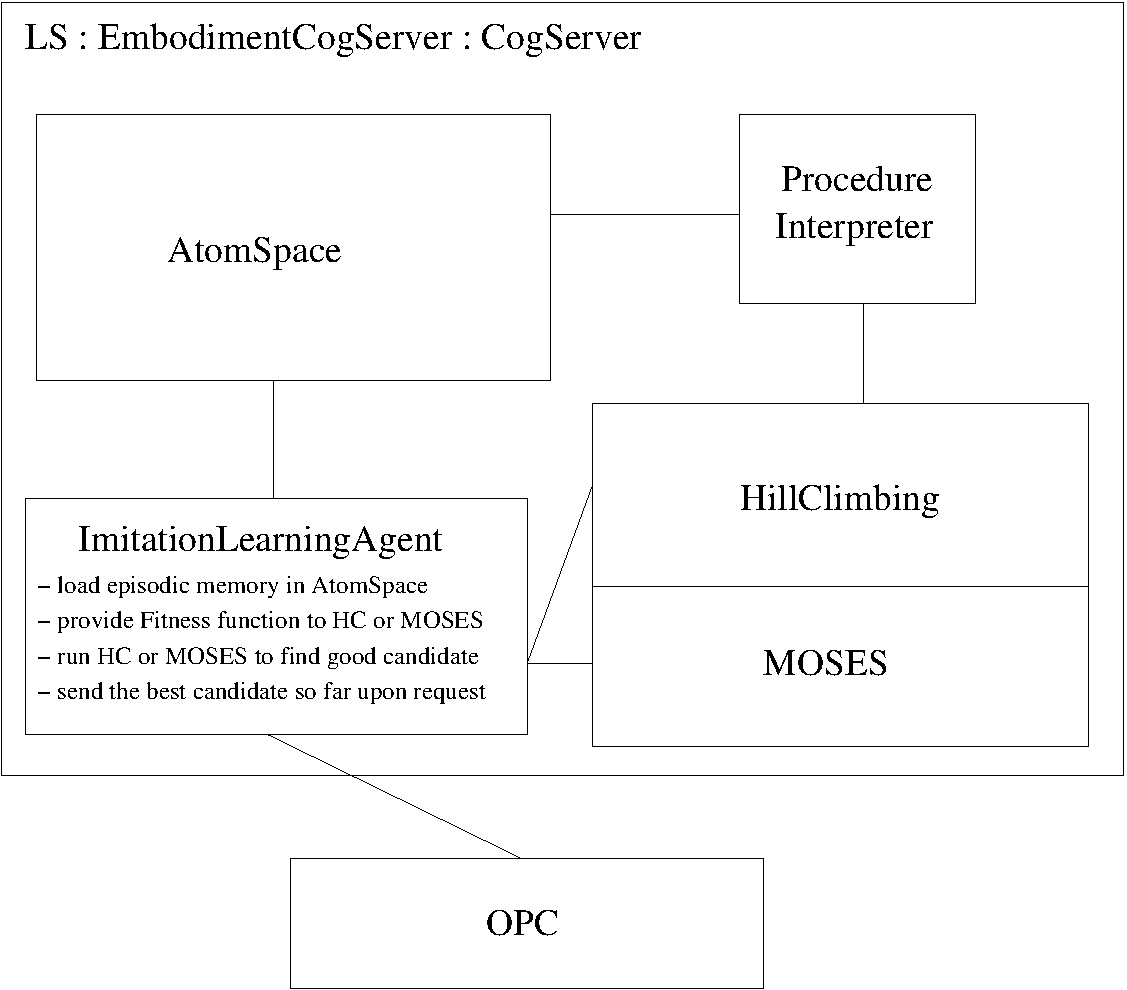
\includegraphics[scale=0.5]{LS.pdf}
}

\end{document}